\documentclass[11pt,paper=a4,answers]{exam}
\usepackage{graphicx,lastpage}
\usepackage{upgreek}
\usepackage{censor}
\usepackage{gensymb}
\usepackage{amsmath}
\usepackage{multicol}
\usepackage{enumitem}
\usepackage{tasks}
\usepackage{adjustbox}
\usepackage{xcolor}
\usepackage{tfrupee}
\setlength{\voffset}{0.25in}
\usepackage{tabularx}
\newcolumntype{Y}{>{\centering\arraybackslash}X}
%==============================================================
% Customise Non-Essential Packages Below
% =============================================================
\usepackage[most]{tcolorbox}
\usepackage{eso-pic}
\usepackage{tikz}
\AddToShipoutPictureBG{%
\begin{tikzpicture}[remember picture,overlay]
\foreach \x in {-8,-4,0,4,8,12,16,20}
\foreach \y in {-8,-4,0,4,8,12,16,20} {
\node[opacity=0.05,rotate=45,anchor=center] at ([xshift=\x cm,yshift=\y cm]current page.center) {%
\begin{minipage}{2cm}
\centering
\includegraphics[width=2cm]{images/logo_black.png}\\
\small preppeo.com
\end{minipage}%
};
}
\end{tikzpicture}%
}
\printanswers

%==============================================================
% Customise Non-Essential Packages Above
% =============================================================
\definecolor{svgray}{rgb}{0.90, 0.90, 0.90}
\graphicspath{{images/}}

\usepackage[normalem]{ulem}
\renewcommand\ULthickness{1pt}   %%---> For changing thickness of underline
\setlength\ULdepth{3.5ex}%\maxdimen ---> For changing depth of underline
\renewcommand{\baselinestretch}{1}
\chead{
\includegraphics[scale=0.1,height=2cm ]{logo.png}
}
\pagestyle{empty}

\pagestyle{headandfoot}
\headrule
\cfoot{W: https://preppeo.com; M: +91-8130711689}

\begin{document}
%==============================================================
% Customise Question paper details below this
% =============================================================
\begin{center}
    \centering
    \renewcommand{\arraystretch}{1.5}
    \begin{tabularx}{\textwidth}{YYY}
    & \normalsize\bf{{\Large{{Quantitative Reasoning}}}} & \\
    By Preppeo & \normalsize\bf{{sat\_lid\_033}} & SAT\\
    \normalsize{{\textbf{{Unit:}}Problem-Solving \& Data Analysis}} & \normalsize{{\textbf{{Chapter:}} Percentages and percentage change}} & \normalsize{{\textbf{{Topic:}} Simple \& Compound Interest}} \\
    \end{tabularx}
\end{center}
\par\noindent\rule{\textwidth}{1pt}
% =============================================================
% Customise Question paper details above this
% =============================================================

\begin{questions}
\pointsinrightmargin
\pointsdroppedatright
\marksnotpoints
\pointpoints{mark}{marks}
\pointformat{\boldmath\themarginpoints}
\bracketedpoints

% =============================================================
% Question Begin
% =============================================================
% --- PART 1: Questions Derived from SAT Screenshots (1-25) ---

% Question 1
% Category: Concept | Difficulty: Medium | Question Type: Multiple Choice
\question
Jeremy deposited $x$ dollars in an investment account on January 1, 2001. The amount of money in the account doubled each year until Jeremy had $480$ in his account on January 1, 2005. Which of the following equations represents the value of the account $V$, in dollars, $t$ years after January 1, 2001?
\begin{tasks}(2)
    \task $V = x+ 2t$
    \task $V = x(2)^t$
    \task $V = 2x^t$
    \task $V = x(t)^2$
\end{tasks}

\begin{solution}
\textbf{Conceptual Explanation:} \\
When a quantity increases by a constant multiplier (in this case, doubling) over equal time intervals, it represents exponential growth. The standard formula for this is $V = P(r)^t$, where $P$ is the initial amount and $r$ is the growth factor.

\vspace{30pt}

\textbf{Calculation and Logic:} \\
1. \textbf{Identify the starting value:} The initial deposit is $x$ dollars. \\
2. \textbf{Identify the growth factor:} "Doubled each year" means the multiplier is 2. \\
3. \textbf{Formulate the equation:} 
   * After 1 year: $x \cdot 2$
   * After 2 years: $(x \cdot 2) \cdot 2 = x(2)^2$
   * After $t$ years: $V = x(2)^t$

\vspace{30pt}

Answer: \colorbox{yellow!100}{B}
\end{solution}

\vspace{60pt}

% Question 2
% Category: Exam level | Difficulty: Hard | Question Type: Multiple Choice
\question
Thomas installed a new stove in his restaurant with an initial value of $800$. He estimates that each year the value of the stove will depreciate by 20% of the previous year’s estimated value. What is the estimated value of the stove exactly 2 years after installation?
\begin{tasks}(2)
    \task $480$
    \task $512$
    \task $556$
    \task $640$
\end{tasks}

\begin{solution}
\textbf{Conceptual Explanation:} \\
Depreciation that is calculated based on the "previous year's value" follows an exponential decay model. Each year, the value is multiplied by a constant decay factor $(1 - \text{rate})$.

\vspace{30pt}

\textbf{Calculation and Logic:} \\
1. \textbf{Identify the decay factor:} A 20% decrease means 80% of the value remains. Multiplier = $0.80$. \\
2. \textbf{Calculate Year 1:} $800 \times 0.80 = 640$. \\
3. \textbf{Calculate Year 2:} $640 \times 0.80 = 512$. \\
Alternatively: $V = 800(0.80)^2 = 800(0.64) = 512$.

\vspace{30pt}

Answer: \colorbox{yellow!100}{B}
\end{solution}

\vspace{60pt}

% Question 3
% Category: Practice | Difficulty: Medium | Question Type: Numeric Entry
\question
An investment of $2,000 earns interest at a constant annual rate. If the account balance is $2,100 after exactly one year, what will the balance be, in dollars, after three years if no additional deposits or withdrawals are made and the account earns simple interest?

\begin{solution}
\textbf{Conceptual Explanation:} \\
Simple interest is calculated only on the initial principal. The amount of interest earned each year remains constant.

\vspace{30pt}

\textbf{Calculation and Logic:} \\
1. \textbf{Find annual interest:} $2100 - 2000 = 100$ dollars per year. \\
2. \textbf{Calculate total interest for 3 years:} $100 \times 3 = 300$. \\
3. \textbf{Find final balance:} $2000 (\text{Principal}) + 300 (\text{Interest}) = 2300$.

\vspace{30pt}

Answer: \colorbox{yellow!100}{2300}
\end{solution}

\vspace{60pt}

% Question 4
% Category: Exam level | Difficulty: Hard | Question Type: Numeric Entry
\question
Jeremy deposited $x$ dollars in his investment account. The amount doubled each year until he had $480$ in the account after 4 years. What is the value of $x$?

\begin{solution}
\textbf{Conceptual Explanation:} \\
To find the initial value in an exponential growth problem, you can work backward from the final amount by performing the inverse operation (halving instead of doubling) for each time period.

\vspace{30pt}

\textbf{Calculation and Logic:} \\
1. \textbf{Value at 4 years:} $480. \\
2. \textbf{Value at 3 years:} $480 / 2 = 240$. \\
3. \textbf{Value at 2 years:} $240 / 2 = 120$. \\
4. \textbf{Value at 1 year:} $120 / 2 = 60$. \\
5. \textbf{Initial Value (0 years):} $60 / 2 = 30.

\vspace{30pt}

Answer: \colorbox{yellow!100}{30}
\end{solution}

\vspace{60pt}

% Question 5
% Category: Concept | Difficulty: Hard | Question Type: Multiple Choice
\question
The value of a collectible item increased by 167% from the end of 2011 to the end of 2012, and then decreased by 16% from the end of 2012 to the end of 2013. Which of the following represents the net percentage increase in value from 2011 to 2013?
\begin{tasks}(2)
    \task 124.28%
    \task 140.28%
    \task 151.00%
    \task 224.28%
\end{tasks}

\begin{solution}
\textbf{Conceptual Explanation:} \\
Successive percentage changes are multiplicative. An increase of 167% corresponds to a multiplier of 2.67, and a decrease of 16% corresponds to a multiplier of 0.84.

\vspace{30pt}
\begin{center}
\begin{tikzpicture}[node distance=3cm, auto]
    \node (p1) [draw, circle] {2011};
    \node (p2) [draw, circle, right of=p1] {2012};
    \node (p3) [draw, circle, right of=p2] {2013};
    \draw[->, thick] (p1) -- node {+167\%} (p2);
    \draw[->, thick] (p2) -- node {-16\%} (p3);
\end{tikzpicture}
\end{center}
\vspace{30pt}

\textbf{Calculation and Logic:} \\
1. \textbf{Combined multiplier:} $2.67 \times 0.84 = 2.2428$. \\
2. \textbf{Convert to percentage:} $(2.2428 - 1) \times 100 = 124.28\%$.

\vspace{30pt}

Answer: \colorbox{yellow!100}{A}
\end{solution}

\vspace{60pt}

% Question 6
% Category: Concept | Difficulty: Medium | Question Type: Multiple Choice
\question
Which of the following is equivalent to increasing a quantity by 110%?
\begin{tasks}(2)
    \task Multiplying by 0.11
    \task Multiplying by 1.10
    \task Multiplying by 2.10
    \task Multiplying by 110
\end{tasks}

\begin{solution}
\textbf{Conceptual Explanation:} \\
A percent increase represents the original 100% plus the additional percentage. Therefore, an increase of 110% results in 210% of the original amount.

\vspace{30pt}

Answer: \colorbox{yellow!100}{C}
\end{solution}

\vspace{60pt}

% Question 7
% Category: Practice | Difficulty: Hard | Question Type: Numeric Entry
\question
The number $w$ is 110% greater than the number $z$. The number $z$ is 55% less than 50. What is the value of $w$?

\begin{solution}
\textbf{Calculation and Logic:} \\
1. \textbf{Calculate z:} $50 \times (1 - 0.55) = 50 \times 0.45 = 22.5$. \\
2. \textbf{Calculate w:} $22.5 \times (1 + 1.10) = 22.5 \times 2.10 = 47.25$.

\vspace{30pt}

Answer: \colorbox{yellow!100}{47.25}
\end{solution}

\vspace{60pt}

% Question 8
% Category: Exam level | Difficulty: Medium | Question Type: Multiple Choice
\question
During a sale, the original prices of all items in a clothing store have been reduced by 20 percent. What is the sale price of a jacket with an original price of $50$?
\begin{tasks}(2)
    \task $12$
    \task $30$
    \task $36$
    \task $40$
\end{tasks}

\begin{solution}
\textbf{Calculation and Logic:} \\
1. \textbf{Multiplier:} $1 - 0.20 = 0.80$. \\
2. \textbf{Sale Price:} $50 \times 0.80 = 40$.

\vspace{30pt}

Answer: \colorbox{yellow!100}{D}
\end{solution}

\vspace{60pt}

% Question 9
% Category: Exam level | Difficulty: Hard | Question Type: Numeric Entry
\question
The regular price of a shirt is $11.70$. The sale price is 80 percent less than the regular price, and the sale price is 30 percent greater than the store's cost for the shirt. What was the store's cost, in dollars, for the shirt?

\begin{solution}
\textbf{Calculation and Logic:} \\
1. \textbf{Find sale price (S):} $11.70 \times (1 - 0.80) = 11.70 \times 0.20 = 2.34$. \\
2. \textbf{Find cost (C):} $2.34 = C \times (1 + 0.30) \Rightarrow 2.34 = 1.3C$. \\
3. \textbf{Solve for C:} $C = 2.34 / 1.3 = 1.80$.

\vspace{30pt}

Answer: \colorbox{yellow!100}{1.80}
\end{solution}

\vspace{60pt}

% Question 10
% Category: Practice | Difficulty: Hard | Question Type: Multiple Choice
\question
37% of the items in a box are green. Of those, 37% are rectangular. Of the green rectangular items, 42% are metal. Which of the following is closest to the percentage of total items in the box that are NOT rectangular green metal items?
\begin{tasks}(2)
    \task 1.16%
    \task 57.50%
    \task 94.25%
    \task 98.84%
\end{tasks}

\begin{solution}
\textbf{Calculation and Logic:} \\
1. \textbf{Percentage of green rectangular metal items:} $0.37 \times 0.37 \times 0.42 \approx 0.0575$ (or 5.75%). \\
2. \textbf{Percentage of items NOT in this group:} $100\% - 5.75\% = 94.25\%$.

\vspace{30pt}

Answer: \colorbox{yellow!100}{C}
\end{solution}

\vspace{60pt}

% Question 11
% Category: Concept | Difficulty: Medium | Question Type: Multiple Choice
\question
The population of City A increased by 7% from 2015 to 2016. If the 2016 population is $k$ times the 2015 population, what is the value of $k$?
\begin{tasks}(2)
    \task 0.07
    \task 0.7
    \task 1.07
    \task 1.7
\end{tasks}

\begin{solution}
\textbf{Calculation and Logic:} \\
An increase of 7% means the new value is $100\% + 7\% = 107\%$ of the old value. In decimal form, this multiplier $k$ is 1.07.

\vspace{30pt}

Answer: \colorbox{yellow!100}{C}
\end{solution}

\vspace{60pt}

% Question 12
% Category: Exam level | Difficulty: Hard | Question Type: Numeric Entry
\question
A bank account earns 2% interest compounded annually. If the initial deposit is $5,000, how much interest is earned after 2 years?

\begin{solution}
\textbf{Calculation and Logic:} \\
1. \textbf{Total balance after 2 years:} $5000 \times (1.02)^2 = 5000 \times 1.0404 = 5202$. \\
2. \textbf{Interest earned:} $5202 - 5000 = 202$.

\vspace{30pt}

Answer: \colorbox{yellow!100}{202}
\end{solution}

\vspace{60pt}

% Question 13
% Category: Practice | Difficulty: Medium | Question Type: Multiple Choice
\question
What is 23% of 100?
\begin{tasks}(2)
    \task 23
    \task 46
    \task 77
    \task 123
\end{tasks}

\begin{solution}
\textbf{Calculation and Logic:} \\
By definition, "percent" means "per hundred." Thus, 23% of 100 is exactly 23.

\vspace{30pt}

Answer: \colorbox{yellow!100}{A}
\end{solution}

\vspace{60pt}

% Question 14
% Category: Practice | Difficulty: Medium | Question Type: Multiple Choice
\question
If 80% of $x$ is 160, what is $x$?
\begin{tasks}(2)
    \task 128
    \task 160
    \task 200
    \task 800
\end{tasks}

\begin{solution}
\textbf{Calculation and Logic:} \\
$0.80x = 160 \Rightarrow x = 160 / 0.80 = 200$.

\vspace{30pt}

Answer: \colorbox{yellow!100}{C}
\end{solution}

\vspace{60pt}

% Question 15
% Category: Concept | Difficulty: Medium | Question Type: Multiple Choice
\question
Which of the following describes the difference between simple and compound interest?
\begin{tasks}(1)
    \task Simple interest is constant addition; compound is constant multiplication.
    \task Simple interest is only on the principal; compound is on principal and accumulated interest.
    \task Simple interest is linear growth; compound interest is exponential growth.
    \task All of the above.
\end{tasks}

\begin{solution}
\textbf{Conceptual Explanation:} \\
Simple interest grows by the same dollar amount each year (linear). Compound interest grows by an increasing dollar amount because it calculates interest on the new total each year (exponential).

\vspace{30pt}

Answer: \colorbox{yellow!100}{D}
\end{solution}

\vspace{60pt}

% Question 16
% Category: Exam level | Difficulty: Hard | Question Type: Numeric Entry
\question
A startup's valuation was $1,000,000$. It increased by 50 percent  in the first year and then decreased by 50 percent  in the second year. What is the valuation after 2 years?

\begin{solution}
\textbf{Calculation and Logic:} \\
1. \textbf{Year 1:} $1,000,000 \times 1.5 = 1,500,000$. \\
2. \textbf{Year 2:} $1,500,000 \times 0.5 = 750,000$.

\vspace{30pt}

Answer: \colorbox{yellow!100}{750000}
\end{solution}

\vspace{60pt}

% Question 17
% Category: Practice | Difficulty: Medium | Question Type: Multiple Choice
\question
If a stock price increases from $40 to $50, what is the percent increase?
\begin{tasks}(2)
    \task 10%
    \task 20%
    \task 25%
    \task 80%
\end{tasks}

\begin{solution}
\textbf{Calculation and Logic:} \\
$\text{Increase} = 50 - 40 = 10$. \\
$\text{Percent Increase} = (10 / 40) \times 100 = 25\%$.

\vspace{30pt}

Answer: \colorbox{yellow!100}{C}
\end{solution}

\vspace{60pt}

% Question 18
% Category: Concept | Difficulty: Medium | Question Type: Multiple Choice
\question
If the expression $P(1.12)^t$ represents an account balance, what is the annual interest rate?
\begin{tasks}(2)
    \task 1.12%
    \task 12%
    \task 112%
    \task $12$
\end{tasks}

\begin{solution}
\textbf{Calculation and Logic:} \\
The growth factor is $1 + r = 1.12$, so $r = 0.12$. In percentage form, this is 12%.

\vspace{30pt}

Answer: \colorbox{yellow!100}{B}
\end{solution}

\vspace{60pt}

% Question 19
% Category: Exam level | Difficulty: Hard | Question Type: Numeric Entry
\question
A car depreciates by 10% each year. If it is currently worth $20,000, how many years will it take for the value to drop below $15,000?

\begin{solution}
\textbf{Calculation and Logic:} \\
1. \textbf{Year 1:} $20000 \times 0.9 = 18000$. \\
2. \textbf{Year 2:} $18000 \times 0.9 = 16200$. \\
3. \textbf{Year 3:} $16200 \times 0.9 = 14580$. (Below 15,000).

\vspace{30pt}

Answer: \colorbox{yellow!100}{3}
\end{solution}

\vspace{60pt}

% Question 20
% Category: Practice | Difficulty: Medium | Question Type: Multiple Choice
\question
If you invest $1,000$ at 5 percent annual simple interest, how much will you have after 10 years?
\begin{tasks}(2)
    \task $1,050$
    \task $1,500$
    \task $1,628$
    \task $2,000$
\end{tasks}

\begin{solution}
\textbf{Calculation and Logic:} \\
1. \textbf{Interest per year:} $1000 \times 0.05 = 50$. \\
2. \textbf{Total interest (10 years):} $50 \times 10 = 500$. \\
3. \textbf{Total balance:} $1000 + 500 = 1500$.

\vspace{30pt}

Answer: \colorbox{yellow!100}{B}
\end{solution}

\vspace{60pt}

% Question 21
% Category: Practice | Difficulty: Medium | Question Type: Multiple Choice
\question
A store marks up a wholesale price of $20$ by 50 percent to get the retail price. What is the retail price?
\begin{tasks}(2)
    \task $10$
    \task $25$
    \task $30$
    \task $40$
\end{tasks}

\begin{solution}
\textbf{Calculation and Logic:} \\
$20 \times (1 + 0.50) = 20 \times 1.5 = 30$.

\vspace{30pt}

Answer: \colorbox{yellow!100}{C}
\end{solution}

\vspace{60pt}

% Question 22
% Category: Exam level | Difficulty: Hard | Question Type: Numeric Entry
\question
If 120% of a number is 54, what is the number?

\begin{solution}
\textbf{Calculation and Logic:} \\
$1.20x = 54 \Rightarrow x = 54 / 1.2 = 45$.

\vspace{30pt}

Answer: \colorbox{yellow!100}{45}
\end{solution}

\vspace{60pt}

% Question 23
% Category: Concept | Difficulty: Medium | Question Type: Multiple Choice
\question
An investment doubles in value every 8 years. Which type of function best models this growth?
\begin{tasks}(2)
    \task Linear
    \task Quadratic
    \task Exponential
    \task Square root
\end{tasks}

\begin{solution}
\textbf{Conceptual Explanation:} \\
Growth defined by a constant doubling time is a classic example of exponential growth.

\vspace{30pt}

Answer: \colorbox{yellow!100}{C}
\end{solution}

\vspace{60pt}

% Question 24
% Category: Exam level | Difficulty: Hard | Question Type: Numeric Entry
\question
An account starts with $100$ and earns 10 percent interest compounded annually. How much interest is earned in the second year?

\begin{solution}
\textbf{Calculation and Logic:} \\
1. \textbf{Year 1 interest:} $100 \times 0.1 = 10$. (Balance = 110). \\
2. \textbf{Year 2 interest:} $110 \times 0.1 = 11$.

\vspace{30pt}

Answer: \colorbox{yellow!100}{11}
\end{solution}

\vspace{60pt}

% Question 25
% Category: Practice | Difficulty: Medium | Question Type: Multiple Choice
\question
A piece of furniture originally costs  200. It is on sale for 15 percent off. What is the sale price?
\begin{tasks}(2)
    \task $30$
    \task $170$
    \task $185$
    \task $230$
\end{tasks}

\begin{solution}
\textbf{Calculation and Logic:} \\
$200 \times (1 - 0.15) = 200 \times 0.85 = 170$.

\vspace{30pt}

Answer: \colorbox{yellow!100}{B}
\end{solution}

% --- PART 2: Advanced Interest and Growth Modeling (26-50) ---

% Question 26
% Category: Exam level | Difficulty: Hard | Question Type: Numeric Entry
\question
An investment account was opened with an initial deposit of \$5,000. The account earns 4\% annual interest compounded semi-annually. What is the total balance in the account, to the nearest dollar, after 3 years if no further deposits or withdrawals are made?

\begin{solution}
\textbf{Conceptual Explanation:} \\
When interest is compounded more than once a year, we use the formula $A = P(1 + \frac{r}{n})^{nt}$. Here, $n$ represents the number of times interest is compounded per year. For semi-annual compounding, $n=2$.

\vspace{30pt}

\textbf{Calculation and Logic:} \\
1. \textbf{Identify variables:} $P = 5000$, $r = 0.04$, $n = 2$, $t = 3$. \\
2. \textbf{Set up the formula:} \\
   \[ A = 5000(1 + \frac{0.04}{2})^{2 \times 3} \]
3. \textbf{Simplify the expression:} \\
   $A = 5000(1.02)^6$ \\
4. \textbf{Calculate the final value:} \\
   $A \approx 5000(1.12616) \approx 5630.8$

\vspace{15pt}

Rounding to the nearest dollar gives 5,631.

\vspace{30pt}

Answer: \colorbox{yellow!100}{5631}
\end{solution}

\vspace{60pt}

% Question 27
% Category: Practice | Difficulty: Medium | Question Type: Multiple Choice
\question
Which of the following functions models the balance $B$ of an account that starts with \$1,200 and earns 1.5\% annual simple interest for $t$ years?
\begin{tasks}(2)
    \task $B = 1200(1.015)^t$
    \task $B = 1200 + 18t$
    \task $B = 1200 + 1.5t$
    \task $B = 1200(0.015)t$
\end{tasks}

\begin{solution}
\textbf{Conceptual Explanation:} \\
Simple interest grows linearly. The interest added each year is a fixed amount based solely on the original principal.

\vspace{30pt}

\textbf{Calculation and Logic:} \\
1. \textbf{Calculate annual interest:} \\
   \$1,200 $\times$ 0.015 = \$18. \\
2. \textbf{Formulate the linear equation:} \\
   Balance = Principal + (Annual Interest $\times$ Years) \\
   $B = 1200 + 18t$.

\vspace{30pt}

Answer: \colorbox{yellow!100}{B}
\end{solution}

\vspace{60pt}

% Question 28
% Category: Concept | Difficulty: Medium | Question Type: Numeric Entry
\question
An investment doubles in value every 10 years. If the initial investment is \$2,500, what will be its value, in dollars, after 30 years?

\begin{solution}
\textbf{Conceptual Explanation:} \\
This problem represents an exponential growth pattern with a specific doubling period. You can determine the number of cycles to find the total multiplier.

\vspace{30pt}
\begin{center}
\begin{tikzpicture}[node distance=3.5cm, auto]
    \node (t0) [draw, thick, rectangle] {Year 0: \$2,500};
    \node (t10) [draw, thick, rectangle, right of=t0] {Year 10: \$5,000};
    \node (t20) [draw, thick, rectangle, below of=t10] {Year 20: \$10,000};
    \node (t30) [draw, thick, rectangle, left of=t20] {Year 30: \$20,000};
    
    \draw[->, ultra thick] (t0) -- node {$\times 2$} (t10);
    \draw[->, ultra thick] (t10) -- node {$\times 2$} (t20);
    \draw[->, ultra thick] (t20) -- node {$\times 2$} (t30);
\end{tikzpicture}
\end{center}
\vspace{30pt}

\textbf{Calculation and Logic:} \\
1. \textbf{Identify cycles:} 30 years $\div$ 10 years = 3 doubling periods. \\
2. \textbf{Apply multiplier:} \$2,500 $\times 2^3$. \\
3. \textbf{Solve:} \$2,500 $\times$ 8 = \$20,000.

\vspace{30pt}

Answer: \colorbox{yellow!100}{20000}
\end{solution}

\vspace{60pt}

% Question 29
% Category: Exam level | Difficulty: Hard | Question Type: Multiple Choice
\question
A tech startup's valuation increased by 40\% in its first year and 50\% in its second year. What was the total percentage increase in valuation over the two-year period?
\begin{tasks}(2)
    \task 90\%
    \task 100\%
    \task 110\%
    \task 210\%
\end{tasks}

\begin{solution}
\textbf{Calculation and Logic:} \\
1. \textbf{Growth factors:} $1.4$ (Year 1) and $1.5$ (Year 2). \\
2. \textbf{Calculate total multiplier:} $1.4 \times 1.5 = 2.1$. \\
3. \textbf{Convert to percentage:} $(2.1 - 1) \times 100 = 110\%$.

\vspace{30pt}

Answer: \colorbox{yellow!100}{C}
\end{solution}

\vspace{60pt}

% Question 30
% Category: Practice | Difficulty: Medium | Question Type: Numeric Entry
\question
A car originally worth \$25,000 depreciates at a rate of 12\% per year. To the nearest dollar, what is the car's value after 5 years?

\begin{solution}
\textbf{Calculation and Logic:} \\
1. \textbf{Multiplier:} $1 - 0.12 = 0.88$. \\
2. \textbf{Equation:} $V = 25000(0.88)^5$. \\
3. \textbf{Solve:} $25000 \times 0.52773 \approx 13193.25$.

\vspace{30pt}

Answer: \colorbox{yellow!100}{13193}
\end{solution}

\vspace{60pt}

% Question 31
% Category: Exam level | Difficulty: Hard | Question Type: Multiple Choice
\question
An account with an initial balance of \$P earns $r$ percent annual interest compounded monthly. Which of the following expressions represents the balance after 2 years?
\begin{tasks}(2)
    \task $P(1 + \frac{r}{100})^{2}$
    \task $P(1 + \frac{r}{1200})^{24}$
    \task $P(1 + \frac{r}{12})^{24}$
    \task $P(1 + \frac{r}{12})^{2}$
\end{tasks}

\begin{solution}
\textbf{Conceptual Explanation:} \\
To convert a whole number percentage $r$ to a monthly decimal rate, divide by 100 (for decimal) and by 12 (for months), resulting in $r/1200$. Over 2 years, there are 24 compounding periods.

\vspace{30pt}

Answer: \colorbox{yellow!100}{B}
\end{solution}

\vspace{60pt}

% Question 32
% Category: Practice | Difficulty: Medium | Question Type: Multiple Choice
\question
How many years will it take for the interest earned on an investment to equal the original principal if the simple interest rate is 8\% per year?
\begin{tasks}(2)
    \task 8 years
    \task 10 years
    \task 12.5 years
    \task 25 years
\end{tasks}

\begin{solution}
\textbf{Calculation and Logic:} \\
$I = Prt$. For $I = P$, then $P = P(0.08)t$. \\
$1 = 0.08t \Rightarrow t = 1 / 0.08 = 12.5$.

\vspace{30pt}

Answer: \colorbox{yellow!100}{C}
\end{solution}

\vspace{60pt}

% Question 33
% Category: Exam level | Difficulty: Hard | Question Type: Numeric Entry
\question
If \$3,000 is invested at 5\% compounded annually, how much more interest is earned after 2 years than if it were invested at 5\% simple interest?

\begin{solution}
\textbf{Calculation and Logic:} \\
1. \textbf{Compound:} $3000(1.05)^2 = 3307.50$ (Interest = \$307.50). \\
2. \textbf{Simple:} $3000 \times 0.05 \times 2 = \$300$ interest. \\
3. \textbf{Difference:} \$307.50 - \$300 = \$7.50.

\vspace{30pt}

Answer: \colorbox{yellow!100}{7.5}
\end{solution}

\vspace{60pt}

% Question 34
% Category: Practice | Difficulty: Medium | Question Type: Multiple Choice
\question
The population of a city grows by 2\% every year. If the population is $P$ now, which expression represents the population in 10 years?
\begin{tasks}(2)
    \task $P + 0.02(10)$
    \task $P(1.02)^{10}$
    \task $P(0.02)^{10}$
    \task $10P(1.02)$
\end{tasks}

\begin{solution}
\textbf{Calculation and Logic:} \\
Population growth is compound growth. Multiplier = $1 + 0.02 = 1.02$. Balance = $P(1.02)^{10}$.

\vspace{30pt}

Answer: \colorbox{yellow!100}{B}
\end{solution}

\vspace{60pt}

% Question 35
% Category: Concept | Difficulty: Medium | Question Type: Numeric Entry
\question
A rare painting was purchased for \$10,000. Every year, its value increases by exactly \$500. After how many years will the painting be worth \$15,000?

\begin{solution}
\textbf{Calculation and Logic:} \\
Total growth needed = \$5,000. \\
Annual growth = \$500. \\
Years = 5000 $\div$ 500 = 10.

\vspace{30pt}

Answer: \colorbox{yellow!100}{10}
\end{solution}

\vspace{60pt}

% Question 36
% Category: Exam level | Difficulty: Hard | Question Type: Multiple Choice
\question
Plan A offers 6\% simple interest. Plan B offers 5\% interest compounded annually. If \$1,000 is invested in each, which is true after 5 years?
\begin{tasks}(1)
    \task Plan A has a higher balance.
    \task Plan B has a higher balance.
    \task Both plans have the same balance.
    \task Plan A is \$100 higher than Plan B.
\end{tasks}

\begin{solution}
\textbf{Calculation and Logic:} \\
1. \textbf{Plan A:} $1000 + (1000 \times 0.06 \times 5) = \$1,300$. \\
2. \textbf{Plan B:} $1000(1.05)^5 \approx \$1,276.28$. \\
3. \$1,300 $>$ \$1,276.28.

\vspace{30pt}

Answer: \colorbox{yellow!100}{A}
\end{solution}

\vspace{60pt}

% Question 37
% Category: Practice | Difficulty: Medium | Question Type: Numeric Entry
\question
How much interest is earned on a \$2,000 deposit at 3\% simple interest over 8 months?

\begin{solution}
\textbf{Calculation and Logic:} \\
Time in years = $8/12 = 2/3$. \\
Interest = $2000 \times 0.03 \times (2/3) = 60 \times (2/3) = 40$.

\vspace{30pt}

Answer: \colorbox{yellow!100}{40}
\end{solution}

\vspace{60pt}

% Question 38
% Category: Exam level | Difficulty: Hard | Question Type: Multiple Choice
\question
The balance of an account after $t$ years is $A = 500(1.08)^t$. Which of the following shows the approximate monthly growth rate?
\begin{tasks}(2)
    \task $A = 500(1.0064)^{12t}$
    \task $A = 500(1.08/12)^{12t}$
    \task $A = 500(1.0064)^{t}$
    \task $A = 500(1.09)^{t/12}$
\end{tasks}

\begin{solution}
\textbf{Calculation and Logic:} \\
$(1.08)^{1/12} \approx 1.0064$. \\
$A = 500((1.08)^{1/12})^{12t} = 500(1.0064)^{12t}$.

\vspace{30pt}

Answer: \colorbox{yellow!100}{A}
\end{solution}

\vspace{60pt}

% Question 39
% Category: Practice | Difficulty: Medium | Question Type: Numeric Entry
\question
What principal is required to earn \$150 in interest at 5\% simple interest over 2 years?

\begin{solution}
\textbf{Calculation and Logic:} \\
$150 = P \times 0.05 \times 2 \Rightarrow 150 = 0.1P$. \\
$P = 150 \div 0.1 = 1500$.

\vspace{30pt}

Answer: \colorbox{yellow!100}{1500}
\end{solution}

\vspace{60pt}

% Question 40
% Category: Concept | Difficulty: Hard | Question Type: Multiple Choice
\question
An investment loses 10\% of its value every month. Which function best models the value of the investment over time?
\begin{tasks}(1)
    \task Linear with a positive slope
    \task Linear with a negative slope
    \task Exponential growth
    \task Exponential decay
\end{tasks}

\begin{solution}
\textbf{Conceptual Explanation:} \\
A constant percentage decrease results in exponential decay.

\vspace{30pt}

Answer: \colorbox{yellow!100}{D}
\end{solution}

\vspace{60pt}

% Question 41
% Category: Exam level | Difficulty: Hard | Question Type: Numeric Entry
\question
If \$1,000 is invested at 10\% compounded annually, what is the balance after 3 years?

\begin{solution}
\textbf{Calculation and Logic:} \\
$1000(1.10)^3 = 1000 \times 1.331 = 1331$.

\vspace{30pt}

Answer: \colorbox{yellow!100}{1331}
\end{solution}

\vspace{60pt}

% Question 42
% Category: Practice | Difficulty: Medium | Question Type: Multiple Choice
\question
A loan of \$400 has a monthly simple interest rate of 1\%. How much interest is owed after 6 months?
\begin{tasks}(2)
    \task \$4
    \task \$24
    \task \$44
    \task \$240
\end{tasks}

\begin{solution}
\textbf{Calculation and Logic:} \\
Monthly interest = \$400 $\times$ 0.01 = \$4. \\
6 months = \$4 $\times$ 6 = \$24.

\vspace{30pt}

Answer: \colorbox{yellow!100}{B}
\end{solution}

\vspace{60pt}

% Question 43
% Category: Exam level | Difficulty: Hard | Question Type: Numeric Entry
\question
A population doubles every 5 years. By what percent does the population increase each year? (Nearest tenth).

\begin{solution}
\textbf{Calculation and Logic:} \\
$(1+r)^5 = 2 \Rightarrow 1+r = 2^{1/5} \approx 1.1487$. \\
$r \approx 0.1487 \Rightarrow 14.9\%$.

\vspace{30pt}

Answer: \colorbox{yellow!100}{14.9}
\end{solution}

\vspace{60pt}

% Question 44
% Category: Practice | Difficulty: Medium | Question Type: Multiple Choice
\question
What is the effective annual rate for 4\% interest compounded quarterly?
\begin{tasks}(2)
    \task 4\%
    \task 4.06\%
    \task 4.12\%
    \task 16\%
\end{tasks}

\begin{solution}
\textbf{Calculation and Logic:} \\
$(1 + 0.04/4)^4 = (1.01)^4 \approx 1.0406$. \\
Rate = 4.06\%.

\vspace{30pt}

Answer: \colorbox{yellow!100}{B}
\end{solution}

\vspace{60pt}

% Question 45
% Category: Practice | Difficulty: Medium | Question Type: Multiple Choice
\question

In the diagram above, which graph represents compound interest?
\begin{tasks}(2)
    \task The straight line
    \task The curve
    \task Both
    \task Neither
\end{tasks}

\begin{solution}
\textbf{Conceptual Explanation:} \\
Compound interest earns "interest on interest," causing it to accelerate upward in a curve (exponential growth).

\vspace{30pt}

Answer: \colorbox{yellow!100}{B}
\end{solution}

\vspace{60pt}

% Question 46
% Category: Exam level | Difficulty: Hard | Question Type: Numeric Entry
\question
An account starts with \$100 and earns 100\% interest compounded annually. What is the balance after 2 years?

\begin{solution}
\textbf{Calculation and Logic:} \\
Multiplier = 2. \\
$100 \times 2^2 = 100 \times 4 = 400$.

\vspace{30pt}

Answer: \colorbox{yellow!100}{400}
\end{solution}

\vspace{60pt}

% Question 47
% Category: Practice | Difficulty: Medium | Question Type: Multiple Choice
\question
A car's value is modeled by $V = 30000(0.85)^t$. What is the annual rate of depreciation?
\begin{tasks}(2)
    \task 0.85\%
    \task 15\%
    \task 85\%
    \task \$30,000
\end{tasks}

\begin{solution}
\textbf{Calculation and Logic:} \\
$1 - r = 0.85 \Rightarrow r = 0.15 = 15\%$.

\vspace{30pt}

Answer: \colorbox{yellow!100}{B}
\end{solution}

\vspace{60pt}

% Question 48
% Category: Exam level | Difficulty: Hard | Question Type: Numeric Entry
\question
If a \$500 investment at 4\% annual simple interest reaches \$600, how many years have passed?

\begin{solution}
\textbf{Calculation and Logic:} \\
Interest = \$100. \\
Annual Interest = \$500 $\times$ 0.04 = \$20. \\
Years = 100 $\div$ 20 = 5.

\vspace{30pt}

Answer: \colorbox{yellow!100}{5}
\end{solution}

\vspace{60pt}

% Question 49
% Category: Concept | Difficulty: Medium | Question Type: Multiple Choice
\question
Which factor most determines how quickly compound interest outpaces simple interest?
\begin{tasks}(1)
    \task The initial principal
    \task The compounding frequency
    \task The length of time
    \task Both frequency and time
\end{tasks}

\begin{solution}
\textbf{Conceptual Explanation:} \\
Both the frequency of compounding and the duration of the investment amplify the exponential effect.

\vspace{30pt}

Answer: \colorbox{yellow!100}{D}
\end{solution}

\vspace{60pt}

% Question 50
% Category: Exam level | Difficulty: Hard | Question Type: Numeric Entry
\question
A bank account grows from \$1,000 to \$1,210 in 2 years with annual compounding. What is the annual interest rate as a percentage?

\begin{solution}
\textbf{Calculation and Logic:} \\
$1210 = 1000(1+r)^2 \Rightarrow 1.21 = (1+r)^2$. \\
$1.1 = 1+r \Rightarrow r = 0.1 = 10\%$.

\vspace{30pt}

Answer: \colorbox{yellow!100}{10}
\end{solution}

% =============================================================
% Question End
% =============================================================

\end{questions}
\begin{center}
\rule{.5\textwidth}{1pt}
\end{center}
\end{document}
